\documentclass{beamer}

%%%%%%%%%%%%%Solarized Theme%%%%%%%%%%%%%%%
\usecolortheme[dark,accent=cyan]{solarized}
\beamertemplatenavigationsymbolsempty
%%%%%Packages%%%%%
\usefonttheme{serif}
\usepackage[T1]{fontenc}
\usepackage[utf8]{inputenc}
\usepackage[english]{babel}
\usepackage{fontawesome}
\usepackage{minted}

\definecolor{DarkGray}{gray}{0.1}
\usemintedstyle{paraiso-dark}


\usepackage{graphicx}
\usepackage{hyperref}
\usepackage{colortbl, xcolor}
\usepackage{booktabs}
\usepackage{amsmath,amsthm, amssymb, latexsym}

\usepackage{tikz}
\usetikzlibrary{er,positioning, calc, patterns, arrows, calc, positioning, arrows, arrows.meta, shapes, automata}
\usetikzlibrary{decorations.pathreplacing, backgrounds, fit}
\tikzset{
    ultra thick/.style={line width=1.6pt},
    % Define standard arrow tip
    >=stealth',
    % Define style for boxes
    punkt/.style={
           ellipse,
           draw=orange,
           ultra thick,
           text width=18em,
           minimum height=8em,
           text centered,
           font=\LARGE},
    % Define arrow style
    pil/.style={
           ->,
           ultra thick,
           draw=orange,
           shorten <=2pt,
           shorten >=2pt,},
    doublepil/.style={
     latex'-latex',
     ultra thick,
     draw=orange,
     shorten <=2pt,
     shorten >=2pt,},
     emojis/.style={
        ellipse,
        text width=17em,
        minimum height=8em,
        text centered,
        font=\LARGE},
}

\usepackage{standalone}
\usepackage{siunitx}
\usetikzlibrary{calc, positioning, arrows, arrows.meta, shapes}
\usetikzlibrary{backgrounds, fit}
\tikzstyle{background}=[orange, rectangle, draw, inner sep=1mm, thick,
           rounded corners=2mm]
\makeatletter
\newcommand{\srcsize}{\@setfontsize{\srcsize}{5pt}{5pt}}
\makeatother

\begin{document}

\begin{frame}
    \begin{center}
        \LARGE{\textbf{\textcolor{orange}{Understanding responses to environments for the Prisoner's Dilemma}}} \\

        \vspace{1.5cm}
        \normalsize{Max Planck Institute}

        \vspace{1cm}
        \normalsize{@NikoletaGlyn}

    \end{center}
\end{frame}

\begin{frame}
    \begin{center}
    
\includegraphics[width=0.24\textwidth]{static/cardiff_uni_logo.png}\hspace{6pt}
    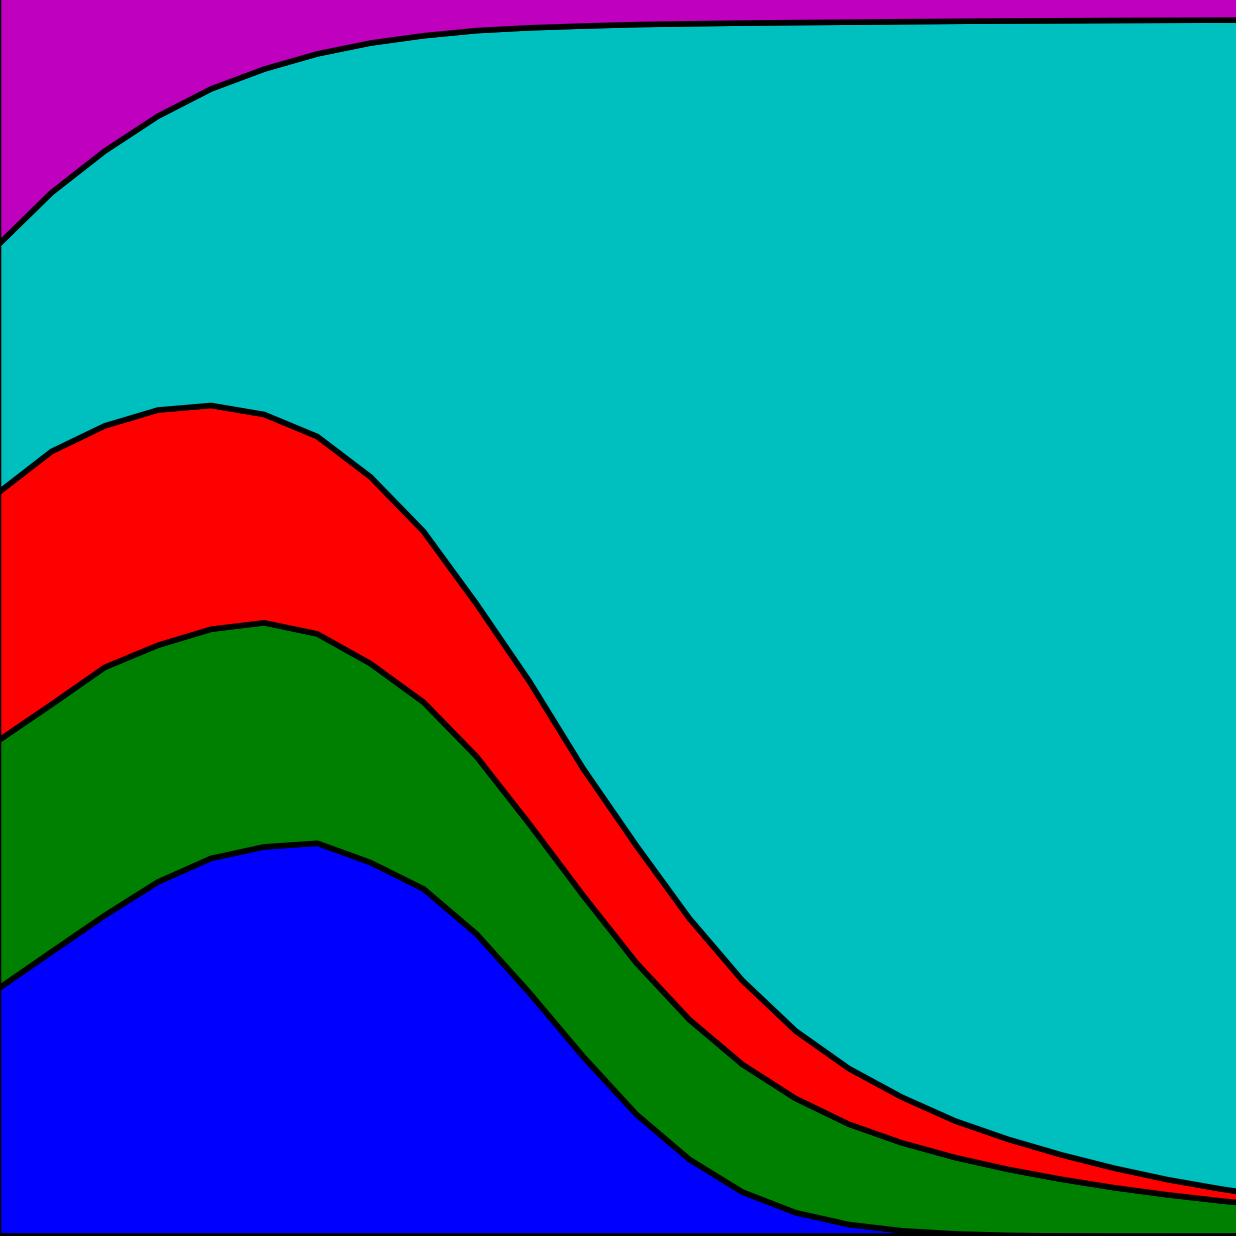
\includegraphics[width=0.24\textwidth, height=0.245\textwidth]{static/axelrod-logo.png}\vspace{10pt}

    \hspace{2pt}
\includegraphics[width=0.24\textwidth]{static/ssi-logo.png} \hspace{1pt}
    
\includegraphics[width=0.24\textwidth]{static/plos-logo.jpg}

    \end{center}
\end{frame}

\begin{frame}
    \begin{center}
    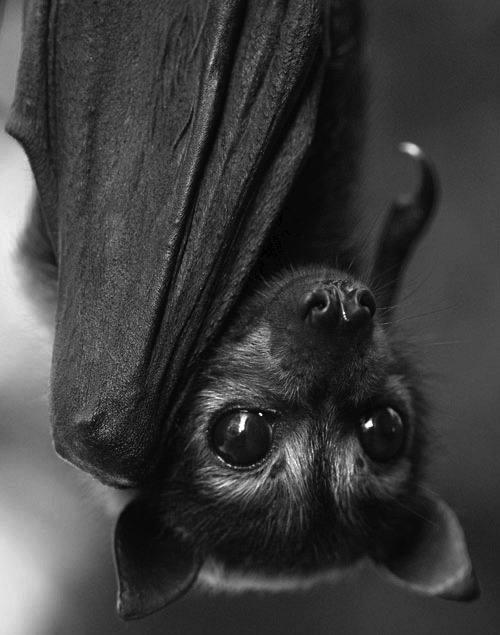
\includegraphics[width=0.5\textwidth]{static/vampire_bat.jpg}\vspace{.7cm}

    \scriptsize{http://rebloggy.com/post/animals-bat-black-and-white-eyes-creepy-horror-gore-halloween-animal-bats-vampir/101865318472}
    \end{center}
\end{frame}

\begin{frame}
    \begin{center}
    \LARGE{
        \begin{equation*}
            S_p =
            \begin{pmatrix}
                3 & 0  \\
                5 & 1
            \end{pmatrix}
            \quad
            S_q =
            \begin{pmatrix}
                3 & 5  \\
                0 & 1
            \end{pmatrix}
        \end{equation*}}
    \end{center}
\end{frame}

\begin{frame}
    \begin{center}
    \includestandalone[width=\textwidth]{static/iterated_prisoners_dilemma}
    \end{center}
\end{frame}

\begin{frame}
    \begin{center}
    \includestandalone[width=\textwidth]{static/structure}
    \end{center}
\end{frame}

\begin{frame}
    \begin{center}
    \textcolor{orange}{\large{\textbf{Bibliometric Study of the Prisoner's Dilemma}}} \vspace{1cm}
    
    
\includegraphics[width=0.10\textwidth]{static/books.png}\hspace{2pt}
\includegraphics[width=0.10\textwidth]{static/pc.png}\hspace{2pt}
\includegraphics[width=0.10\textwidth]{static/chart.png}
    \end{center}
\end{frame}

\begin{frame}
    \begin{center}
    \includestandalone[width=.7\textwidth]{static/arcas_diagram}
    \end{center}
\end{frame}

\begin{frame}
    \begin{center}
    \small{title="prisoner's dilemma" OR abstract="prisoner's dilemma"}\\
    
    \vspace{-.50cm}
    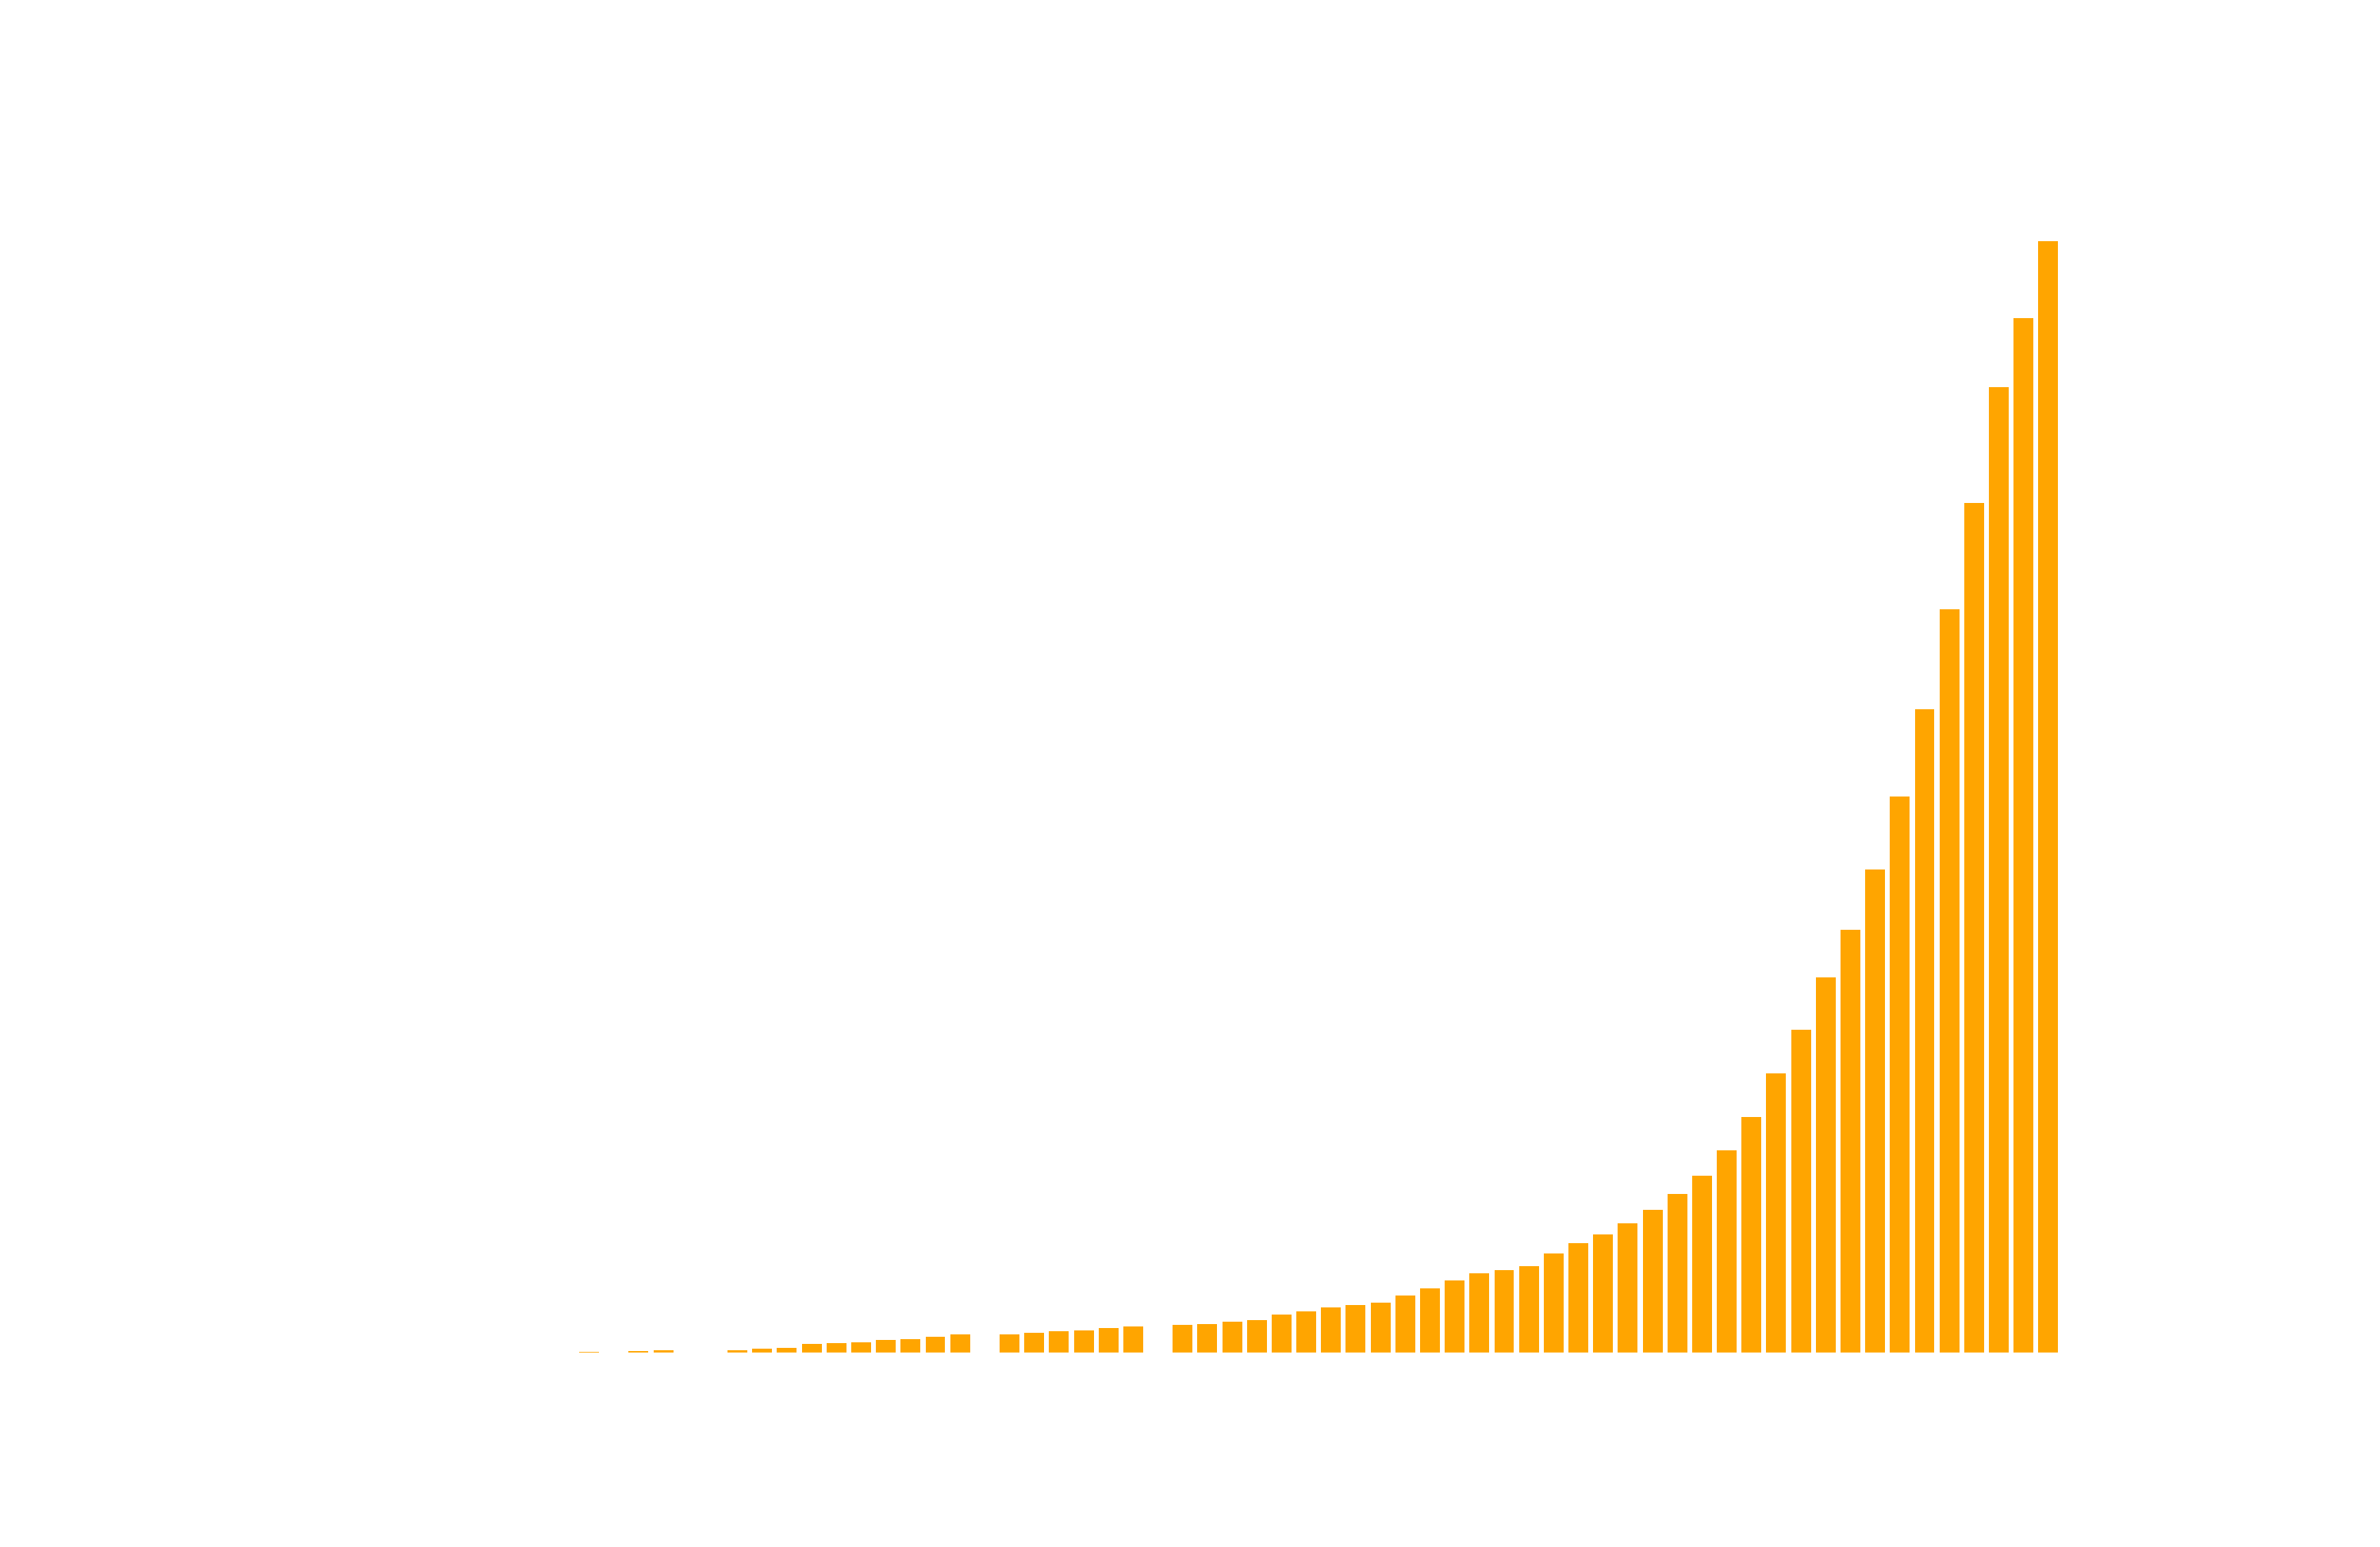
\includegraphics[width=\textwidth]{static/articles.png}
    \end{center}
\end{frame}

\begin{frame}
    \begin{center}
    \includestandalone[width=\textwidth]{static/lda}
    \end{center}
\end{frame}

\begin{frame}
    \begin{center}
    \includestandalone[width=\textwidth]{static/topics}
    \end{center}
\end{frame}

% \begin{frame}
%     \begin{center}
%         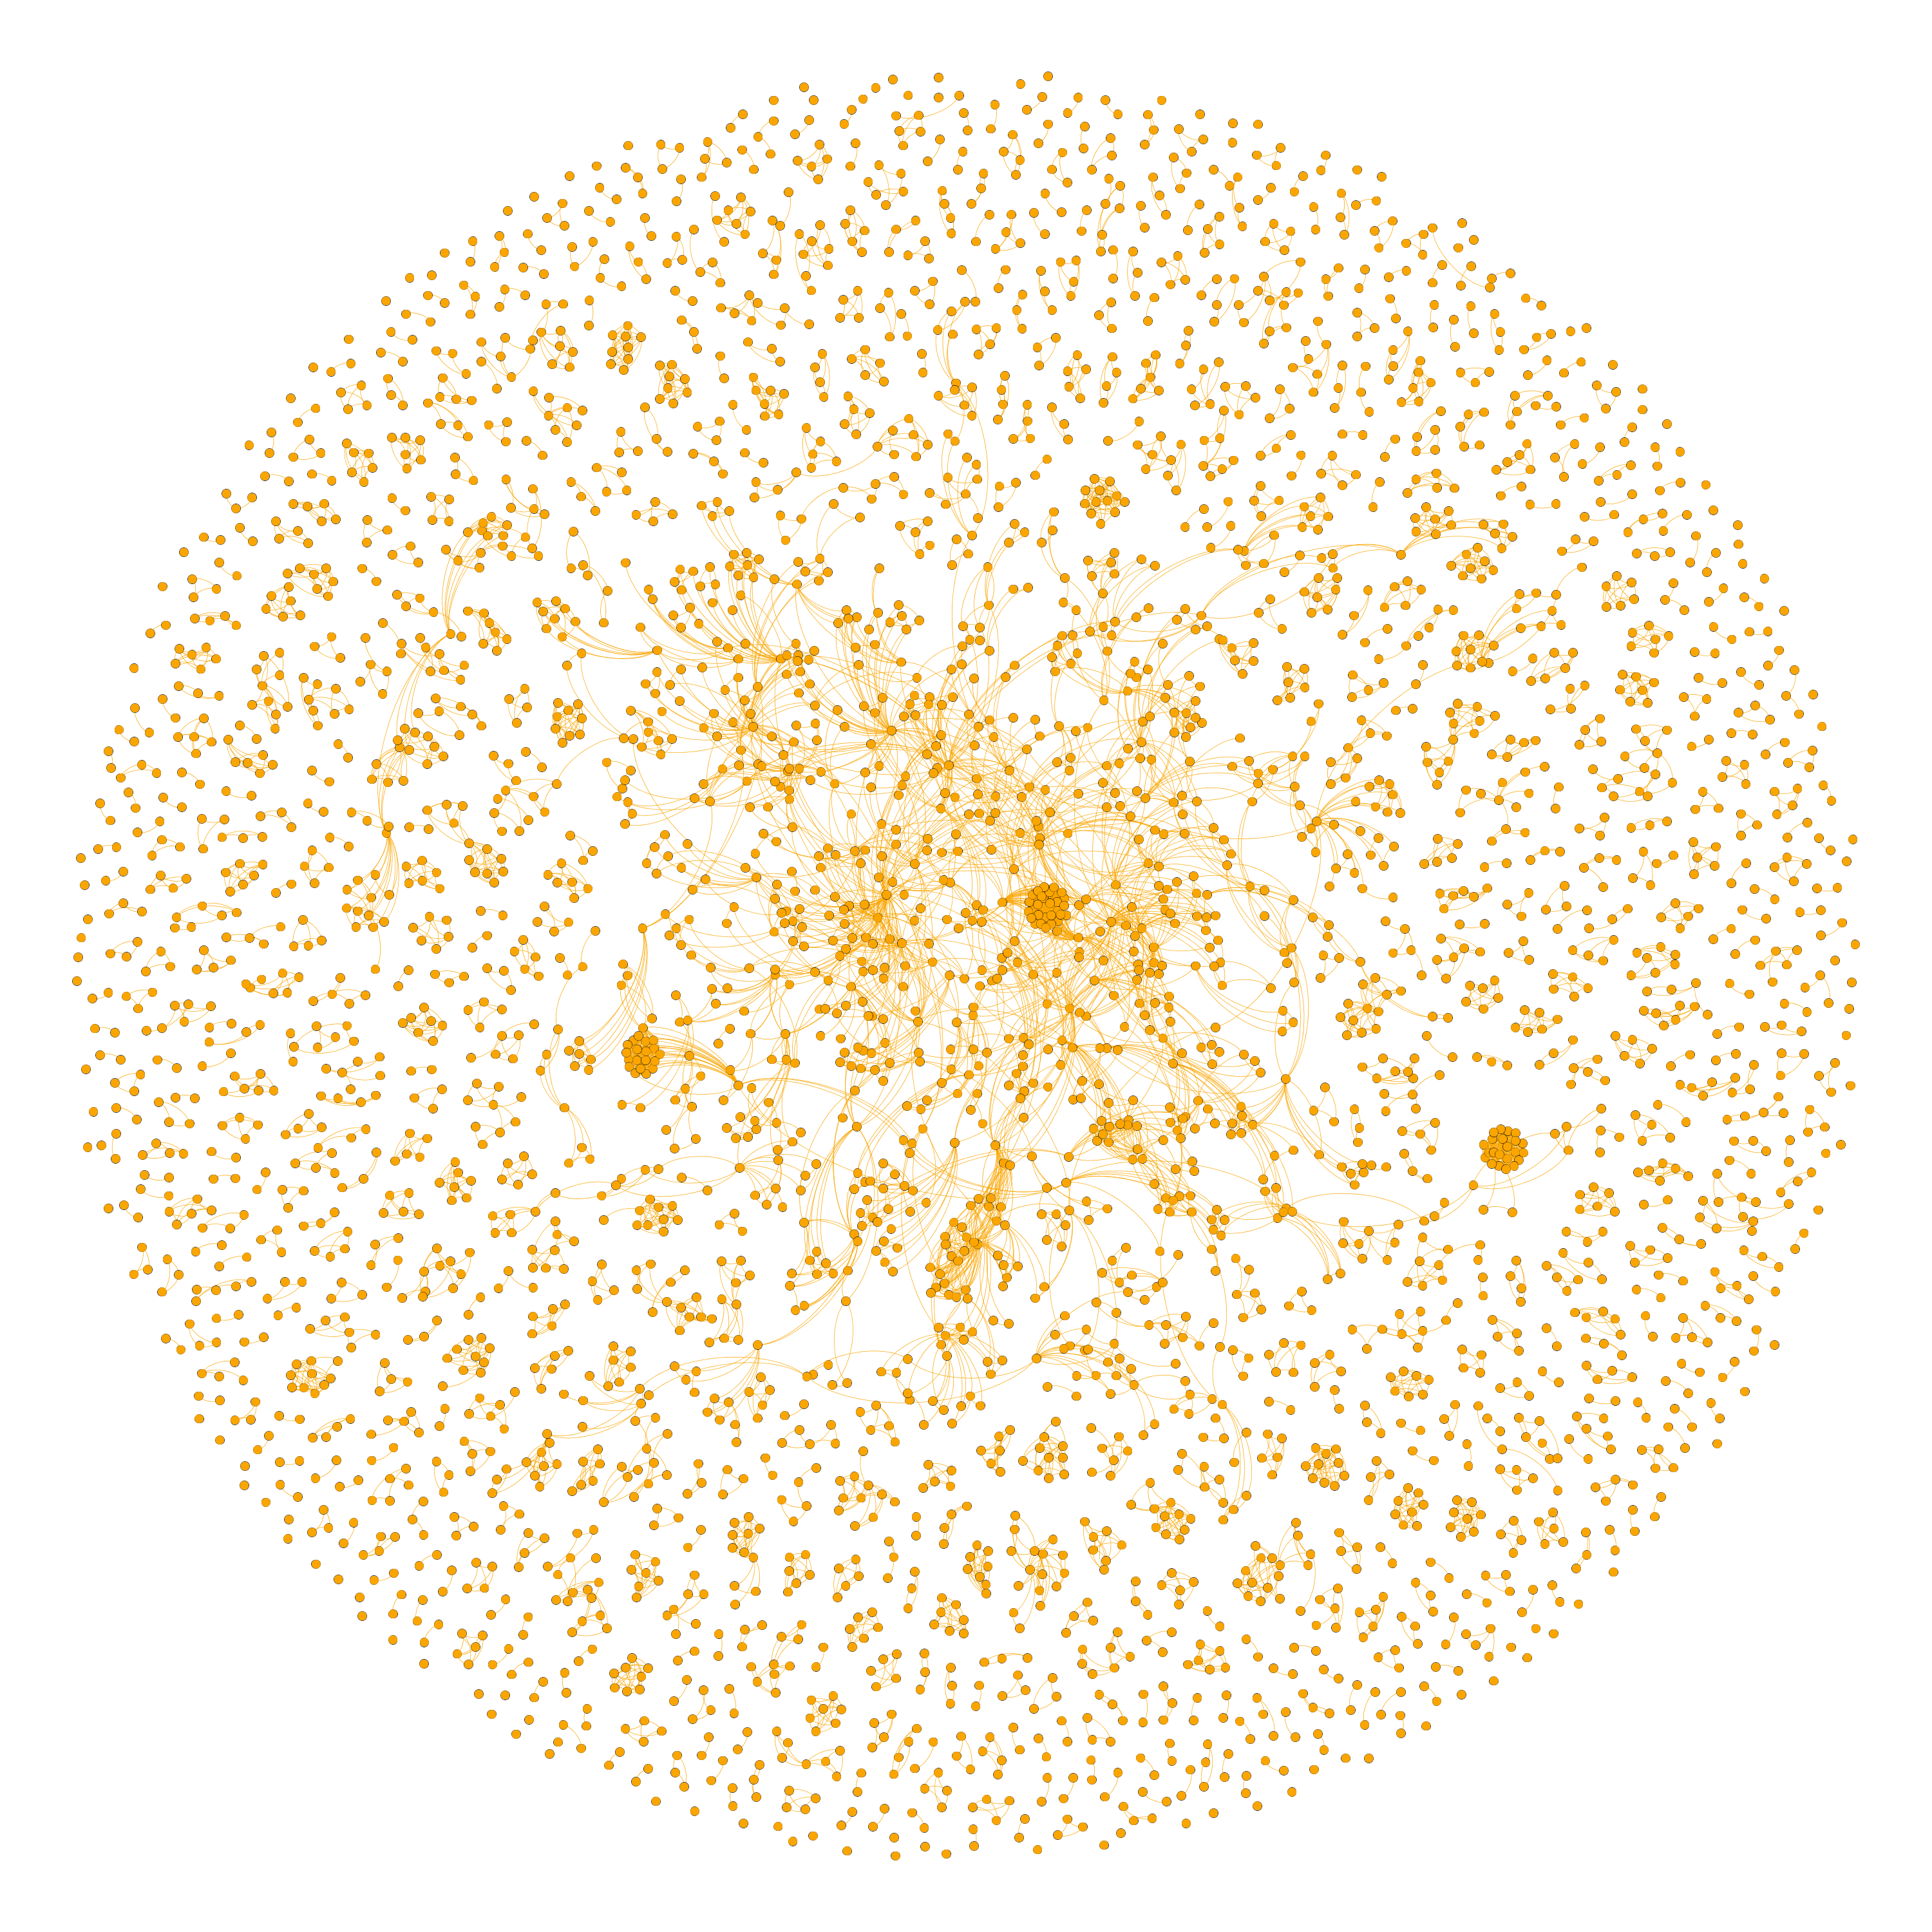
\includegraphics[width=.7\textwidth]{static/pd.png}
%     \end{center}
% \end{frame}

\begin{frame}
    \begin{center}
        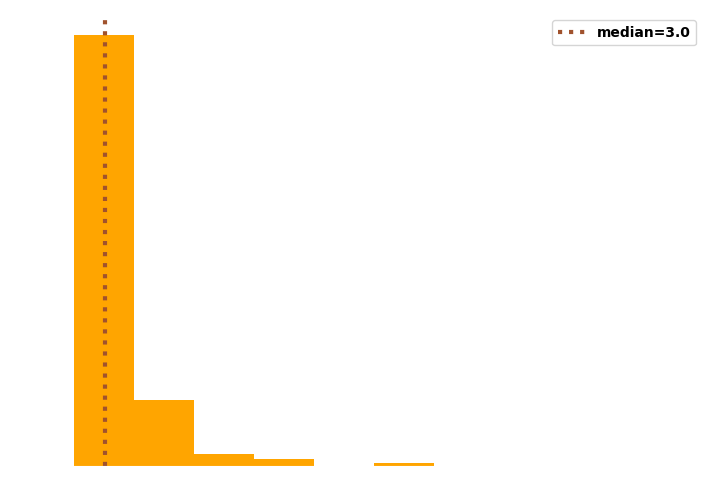
\includegraphics[width=.7\textwidth]{static/degree_dist.png}
    \end{center}
\end{frame}

\begin{frame}
    \begin{center}
        \large{``A bibliometric study of research topics, collaboration and influence in the field of the Iterated Prisoner's Dilemma"} \\ \vspace{.5cm}
        \footnotesize{Nikoleta E. Glynatsi, Vincent A. Knight} \\ \vspace{.5cm}
        \footnotesize{https://arxiv.org/abs/1911.06128}
    \end{center}
\end{frame}

%%%%%%%%%%%%%%%%%%%%%%%%%%%%%%%%END-BIBLIOMETRIC%%%%%%%%%%%%%%%%%%%%%%%%%%%%%%%%
\begin{frame}
    \begin{center}
    \textcolor{orange}{\large{\textbf{Meta Analysis of Tournaments}}} \vspace{1cm}

    
\includegraphics[width=0.10\textwidth]{static/look.png}\hspace{2pt}
\includegraphics[width=0.10\textwidth]{static/bar.png}
    \end{center}
\end{frame}

\begin{frame}
    \begin{center}
        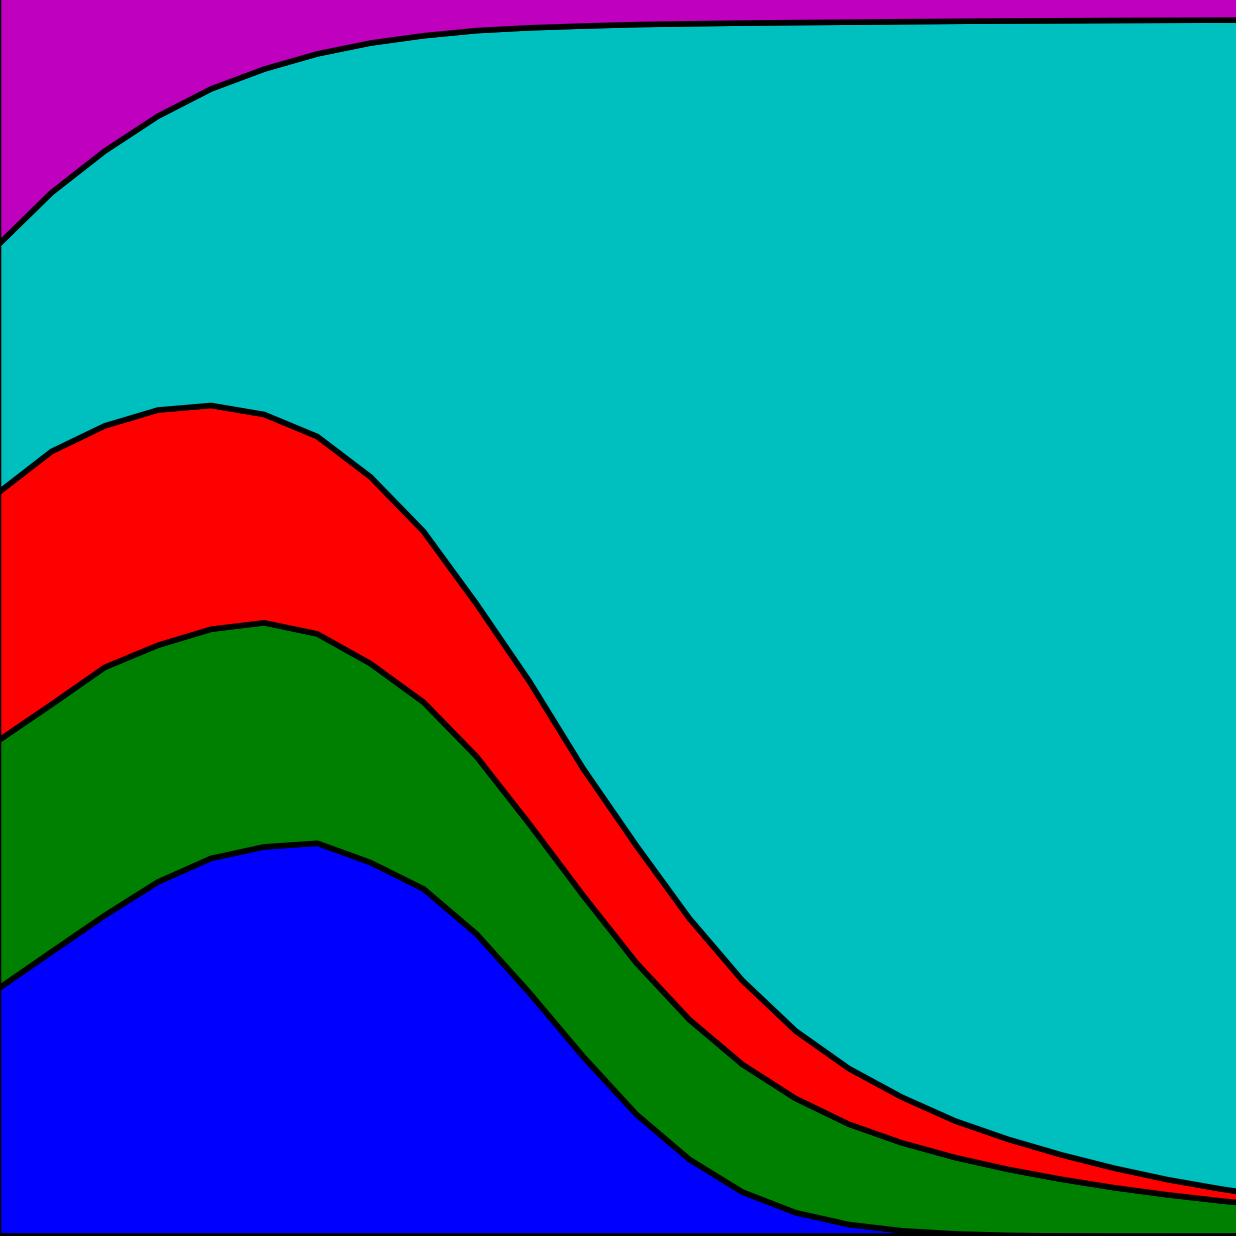
\includegraphics[width=.25\textwidth]{static/axelrod-logo.png}
    \end{center}
\end{frame}

\begin{frame}
    \begin{center}
    \Large{\textbf{195}} \small{strategies in} \Large{\textbf{45686}} \small{tournaments}
    \end{center}
\end{frame}

\begin{frame}
    \begin{center}
        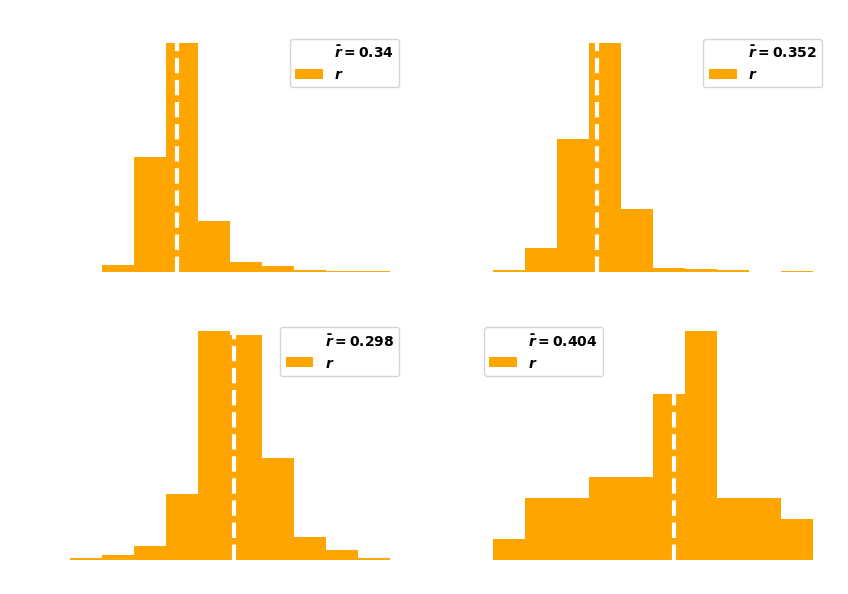
\includegraphics[width=\textwidth]{static/tit_for_tat_r_distributions.png}
    \end{center}
\end{frame}

\begin{frame}
    \begin{center}
        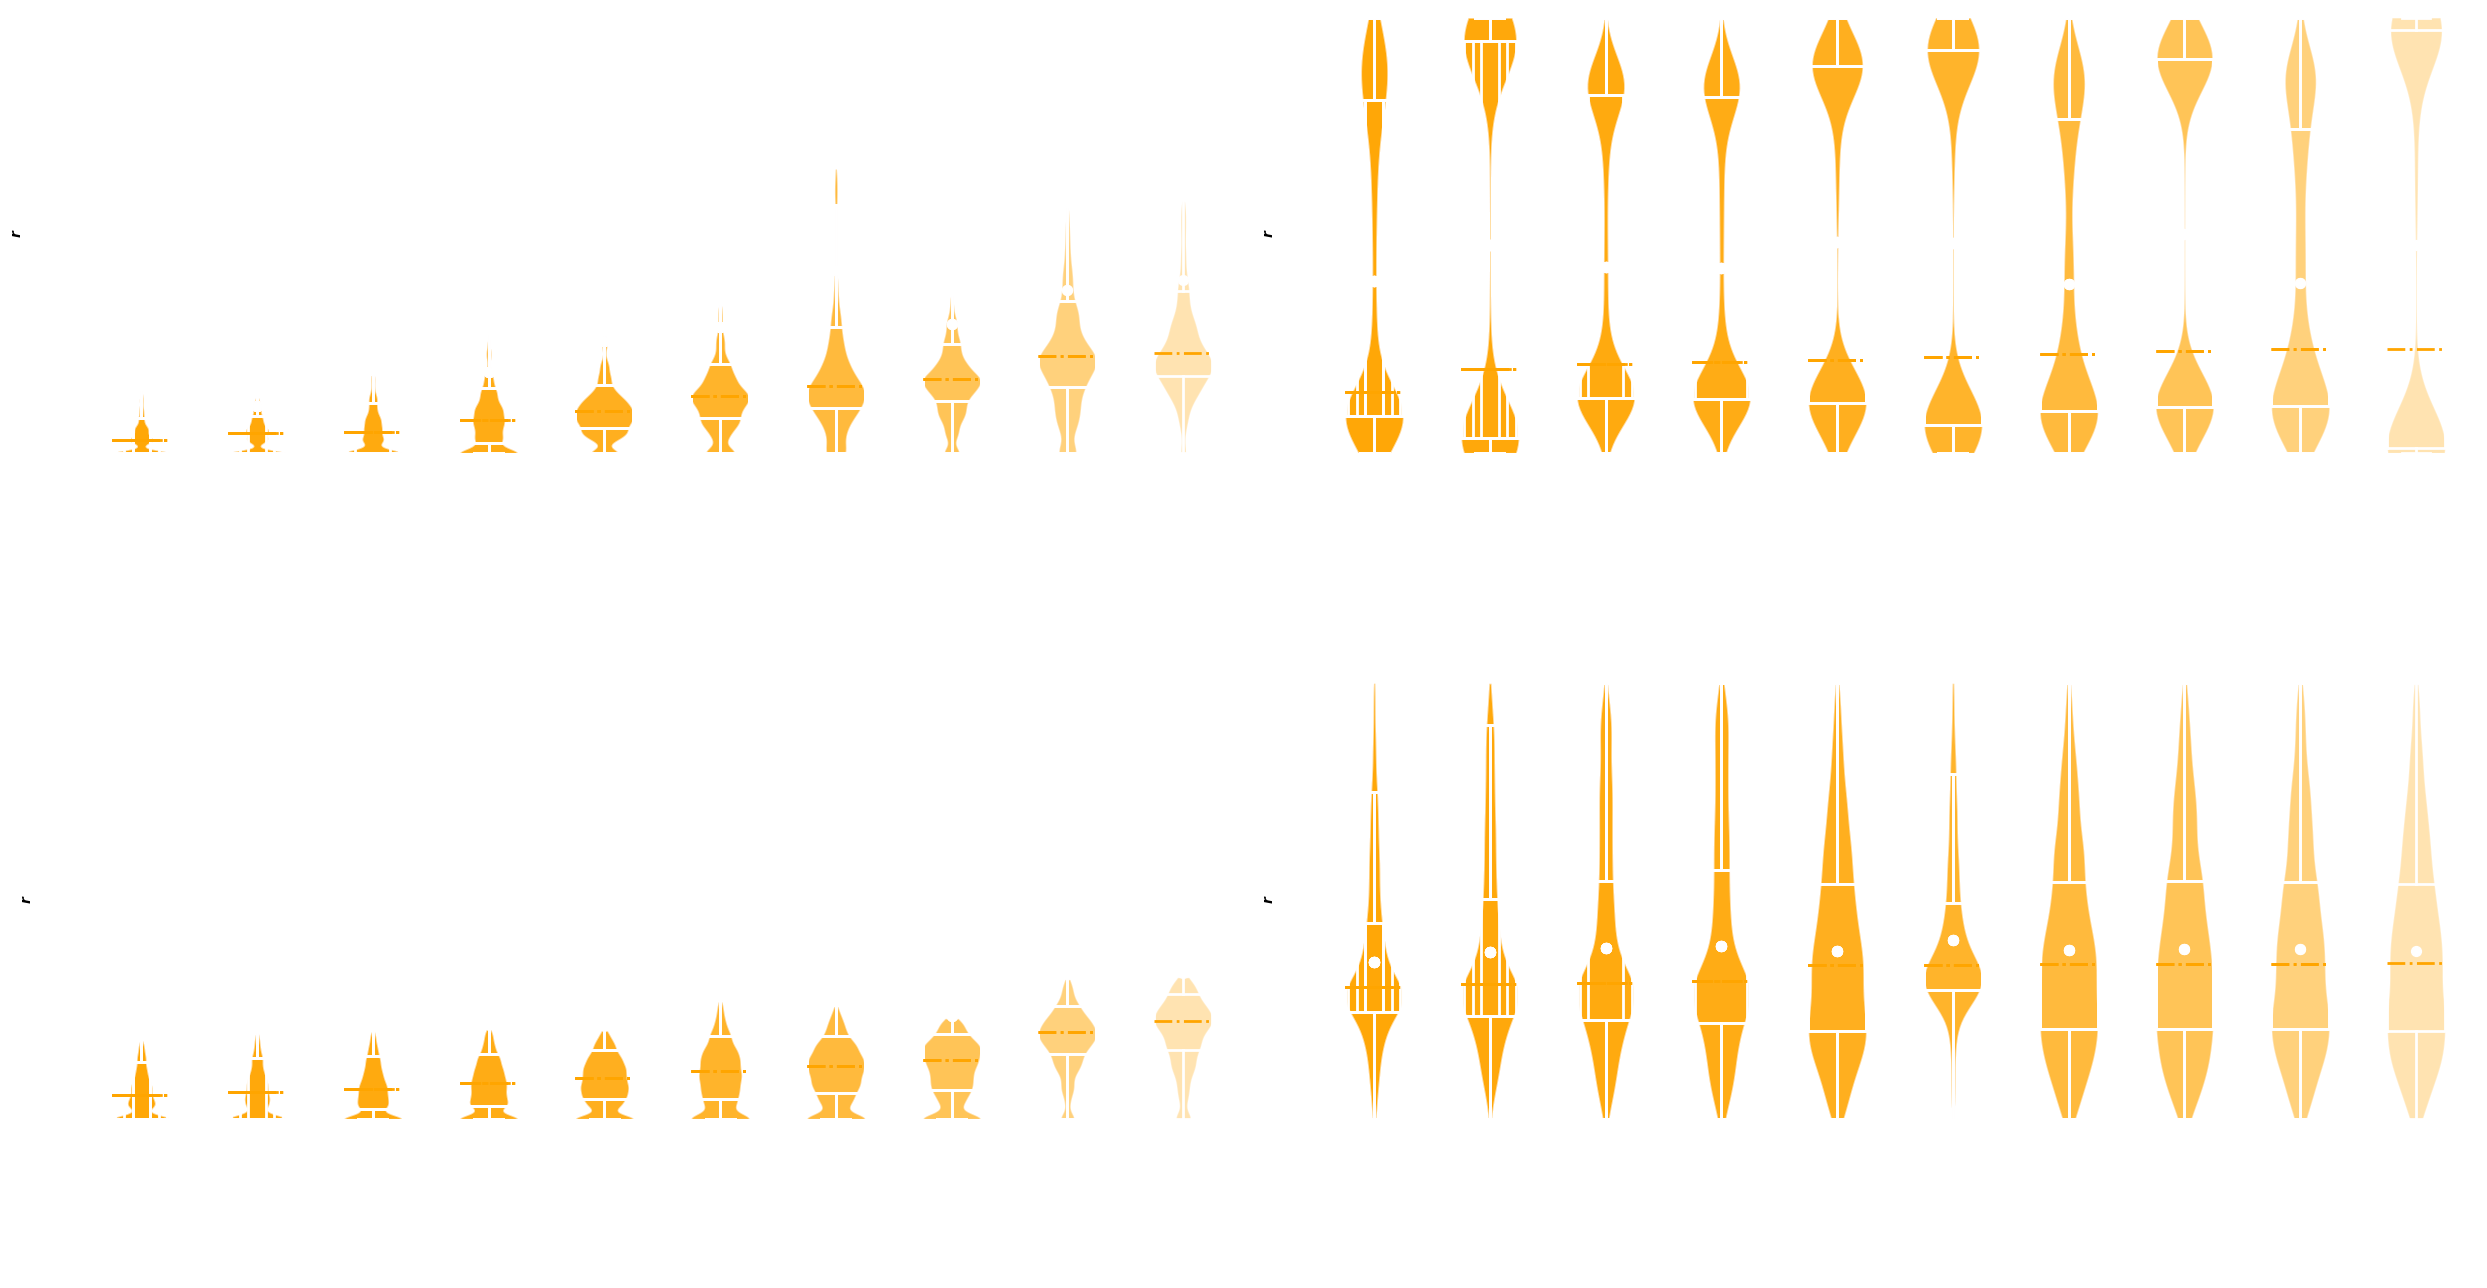
\includegraphics[width=\textwidth]{static/performances.png}
    \end{center}
\end{frame}

\begin{frame}
    \begin{center}
    \Large{\textbf{Evolved HMM 5 ?}}
    \end{center}
\end{frame}

\begin{frame}
    \begin{center}
        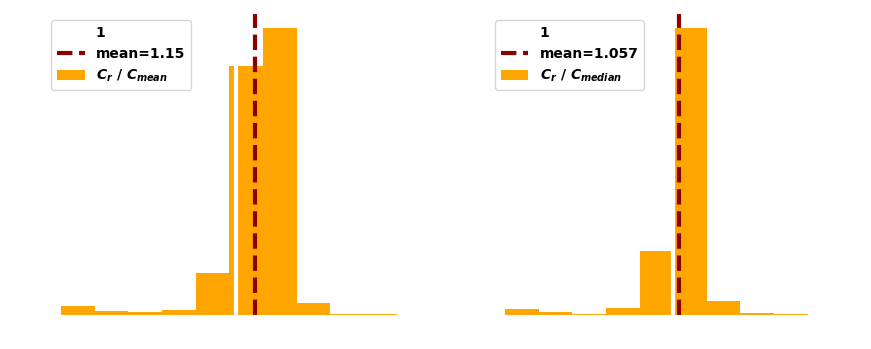
\includegraphics[width=.8\textwidth]{static/features.png}
    \end{center}
\end{frame}


\begin{frame}
    \begin{center}
        \large{``A meta analysis of tournaments and an evaluation of performance in the Iterated Prisoner's Dilemma"} \\ \vspace{.5cm}
        \footnotesize{Nikoleta E. Glynatsi, Vincent A. Knight} \\ \vspace{.5cm}
        \footnotesize{arXiv:2001.05911}
    \end{center}
\end{frame}

%%%%%%%%%%%%%%%%%%%%%%%%%%%%%%%%%%%%END-META%%%%%%%%%%%%%%%%%%%%%%%%%%%%%%%%%%%%
\begin{frame}
    \begin{center}
    \textcolor{orange}{\large{\textbf{Best Response Memory One Strategies}}} \vspace{1cm}

    
\includegraphics[width=0.10\textwidth]{static/look.png}\hspace{2pt}
\includegraphics[width=0.10\textwidth]{static/memone.png}
    \end{center}
\end{frame}

\begin{frame}
    \begin{center}
    \includestandalone[width=.7\textwidth]{static/markov_chain}
    \end{center}
\end{frame}

\begin{frame}
    \begin{center}
    \includestandalone[width=.9\textwidth]{static/problem_maximisation}
    \end{center}
\end{frame}

\begin{frame}
    \begin{center}
    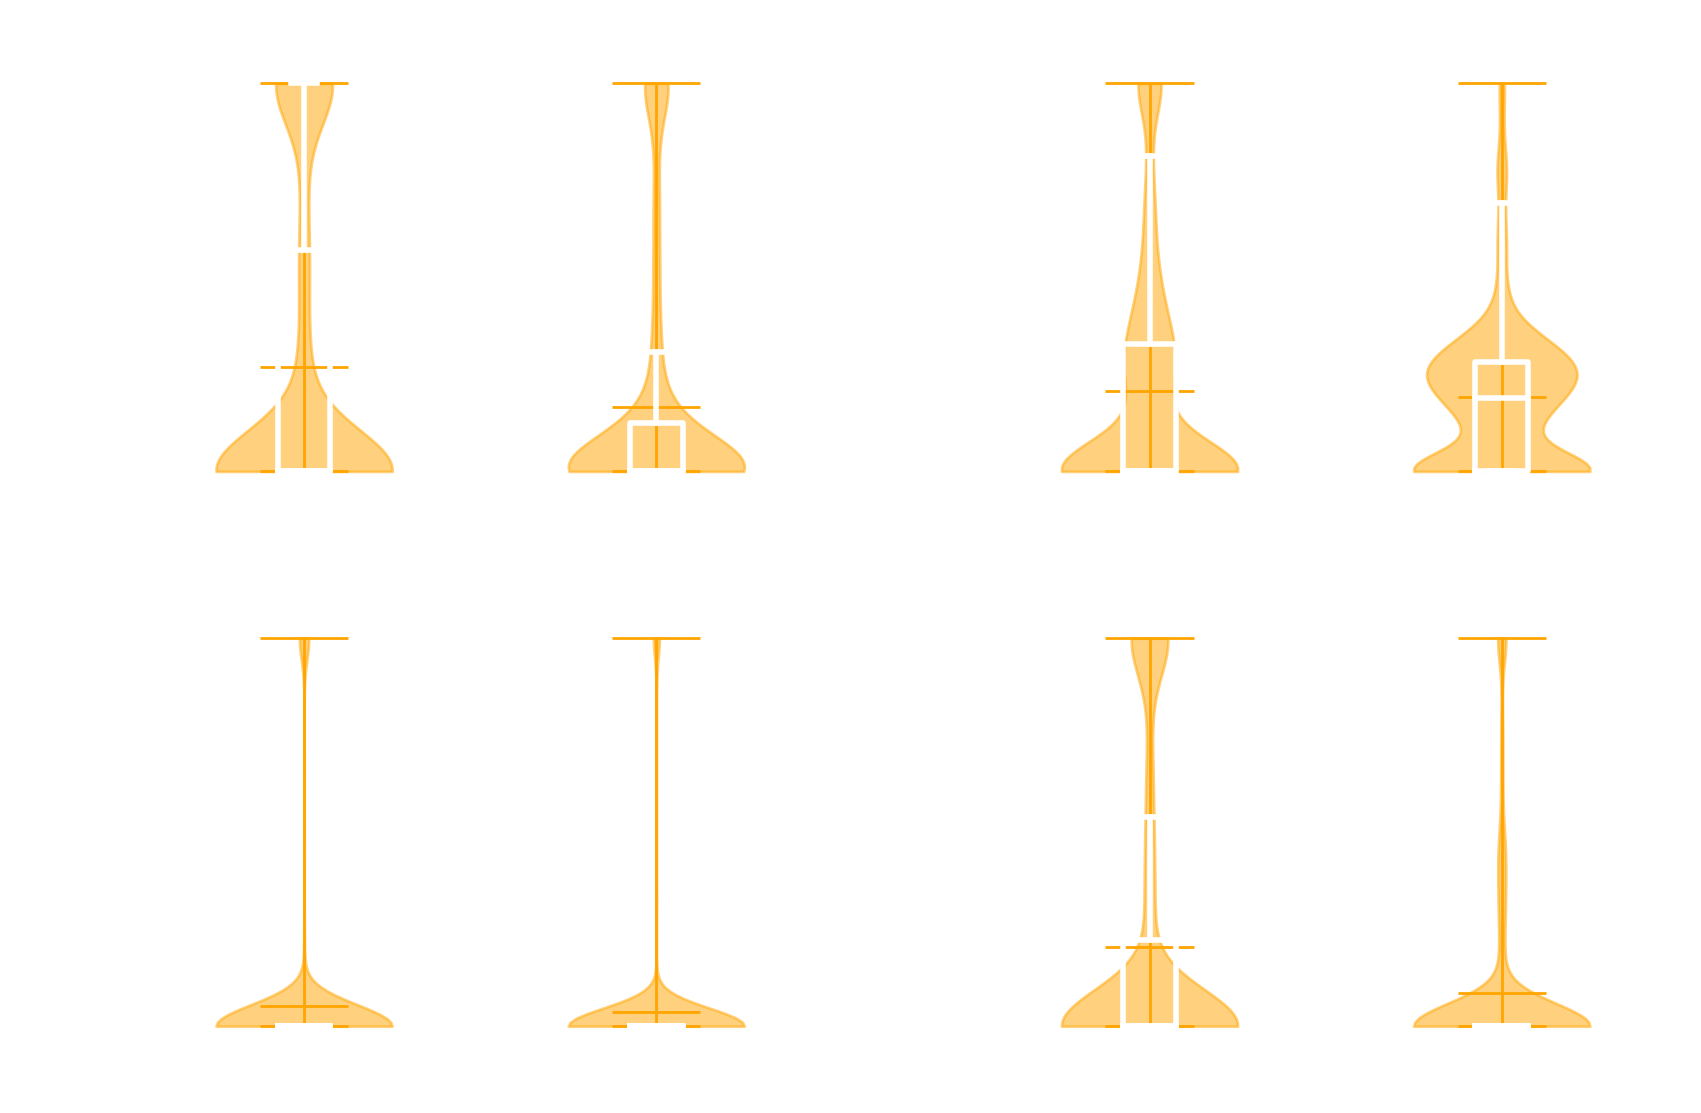
\includegraphics[width=.8\textwidth]{static/mem_one_violin.png}
    \end{center}
\end{frame}

\begin{frame}
    \begin{center}
        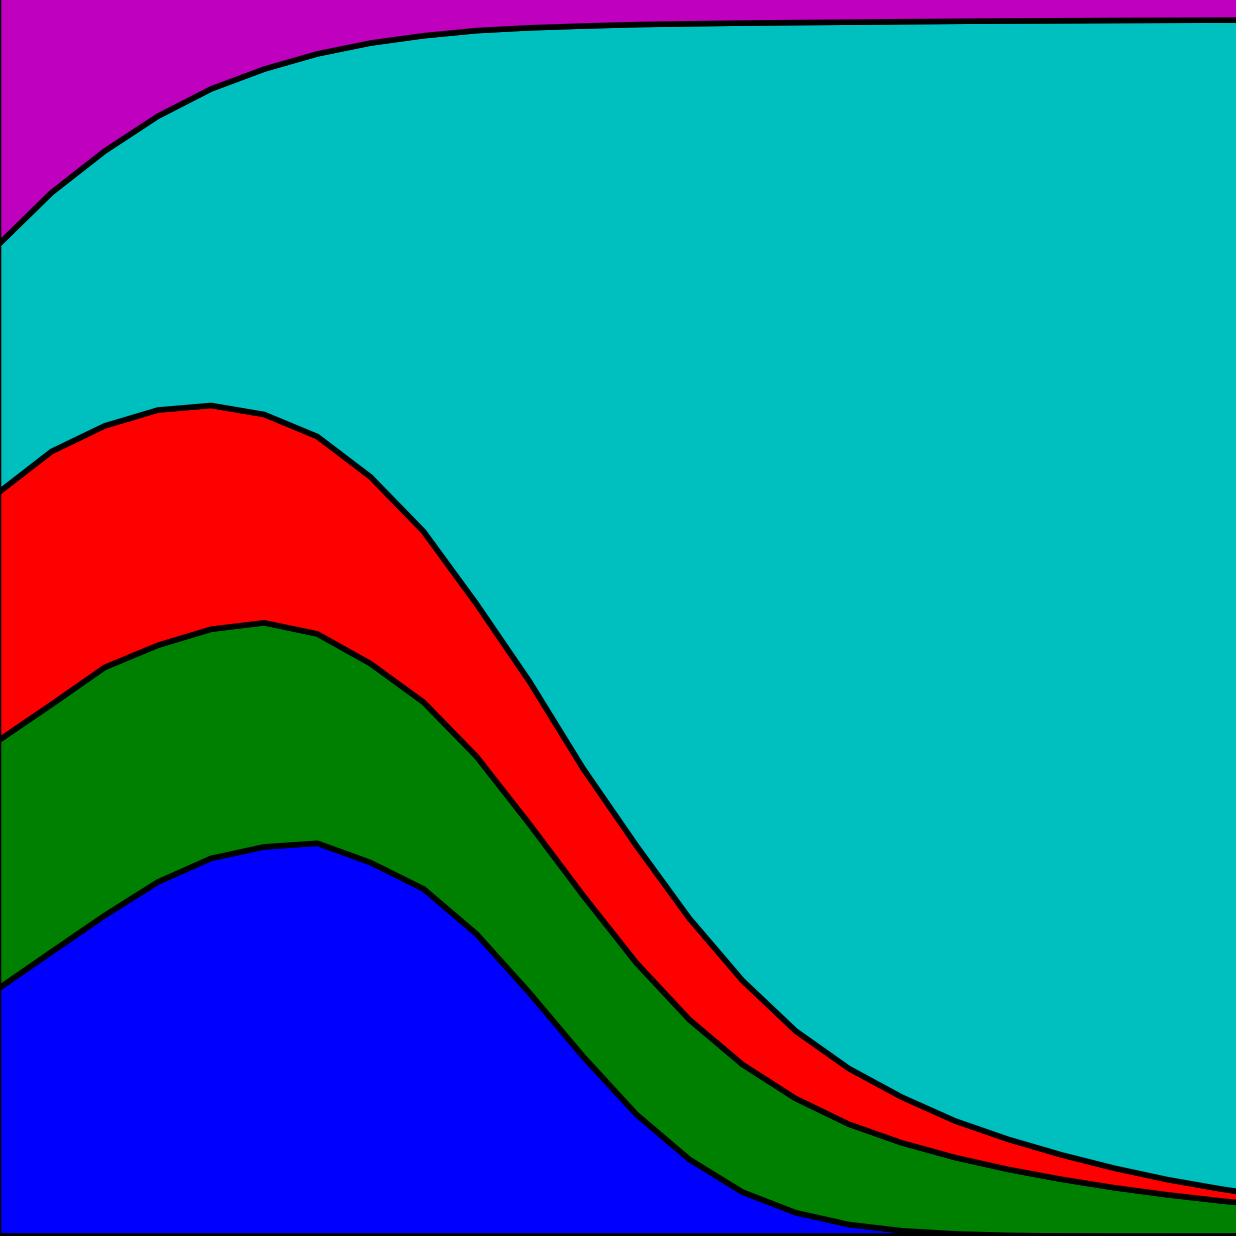
\includegraphics[width=.25\textwidth]{static/axelrod-logo.png}
    \end{center}
\end{frame}

\begin{frame}
    \begin{center}
    
\includegraphics[width=.8\textwidth]{static/mem_one_against_longer_memory.png}
    \end{center}
\end{frame}

\begin{frame}
    \begin{center}
        \large{``Stability of defection, optimisation of strategies and the limits of memory in the Prisoner's Dilemma "} \\ \vspace{.5cm}
        \footnotesize{Nikoleta E. Glynatsi, Vincent A. Knight} \\ \vspace{.5cm}
        \footnotesize{arXiv:1911.12112}
    \end{center}
\end{frame}

%%%%%%%%%%%%%%%%%%%%%%%%%%%%%%%%%%%END-MEMONE%%%%%%%%%%%%%%%%%%%%%%%%%%%%%%%%%%%
\begin{frame}
    \begin{center}
    \textcolor{orange}{\large{\textbf{Best Response Sequences}}} \vspace{1cm}

    
\includegraphics[width=0.10\textwidth]{static/sequence.png}\hspace{2pt}
\includegraphics[width=0.10\textwidth]{static/lstm.png}
    \end{center}
\end{frame}

\begin{frame}
    \begin{center}
    \includestandalone[width=.9\textwidth]{static/tft_vs_defector}
    \end{center}
\end{frame}


\begin{frame}
    \begin{center}
    \includestandalone[width=.95\textwidth]{static/tft_vs_best_response}
    \end{center}
\end{frame}

\begin{frame}
    \begin{center}
    \includestandalone[width=.9\textwidth]{static/best_sequences}
    \end{center}
\end{frame}
%%%%%%%%%%%%%%%%%%%%%%%%%%%%%%%%%%END-SEQUENCES%%%%%%%%%%%%%%%%%%%%%%%%%%%%%%%%%%
\begin{frame}
    \begin{center}
        \textcolor{orange}{\large{\textbf{Recurrent Neural Network Player}}} \vspace{1cm}
    
        
\includegraphics[width=0.10\textwidth]{static/look.png}\hspace{2pt}
\includegraphics[width=0.10\textwidth]{static/bar.png}
    \end{center}
\end{frame}

\begin{frame}
    \begin{center}
    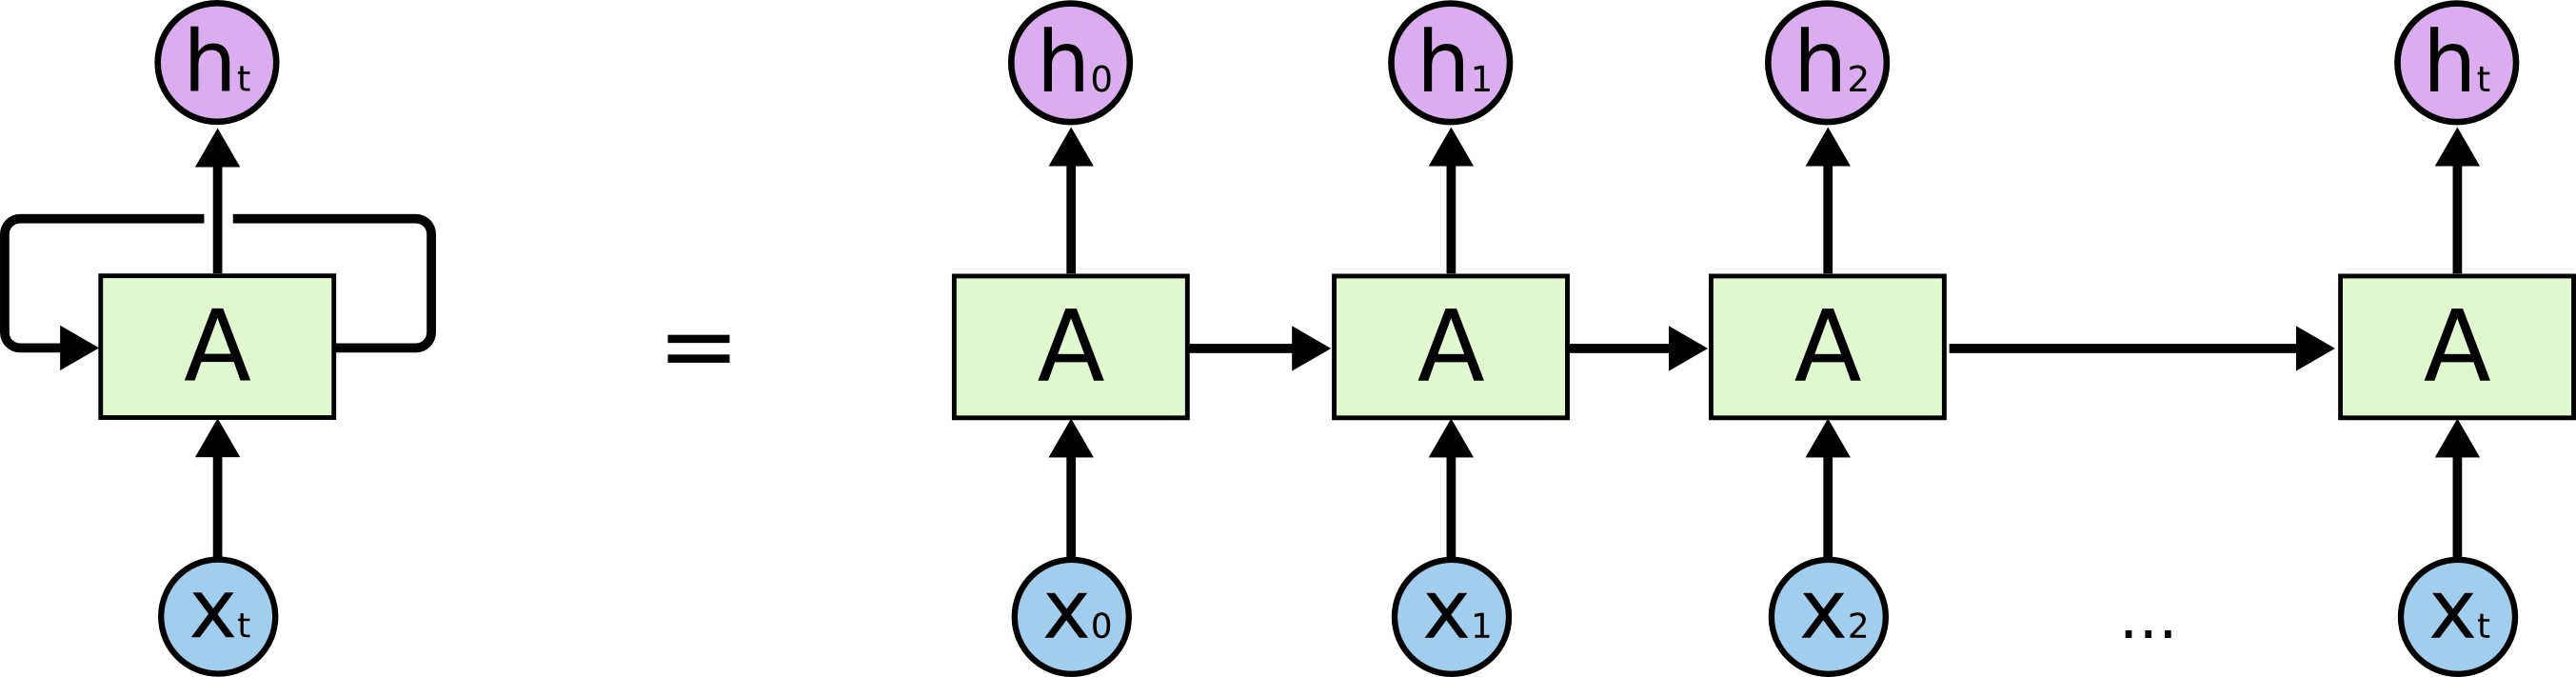
\includegraphics[width=.9\textwidth]{static/Diagram_lstm.png}
    \end{center}
\end{frame}

\begin{frame}
    \begin{center}
    Performance violin plot
    \end{center}
\end{frame}
%%%%%%%%%%%%%%%%%%%%%%%%%%%%%%%%%%%%END-LSTM%%%%%%%%%%%%%%%%%%%%%%%%%%%%%%%%%%%%
\begin{frame}
    \begin{center}
        \begin{itemize}
            \item Point 1
            \item Point 2
            \item Point 3
            \item Point 4
            \item Point 5
        \end{itemize}
    \end{center}
\end{frame}

\begin{frame}
    \begin{center}
    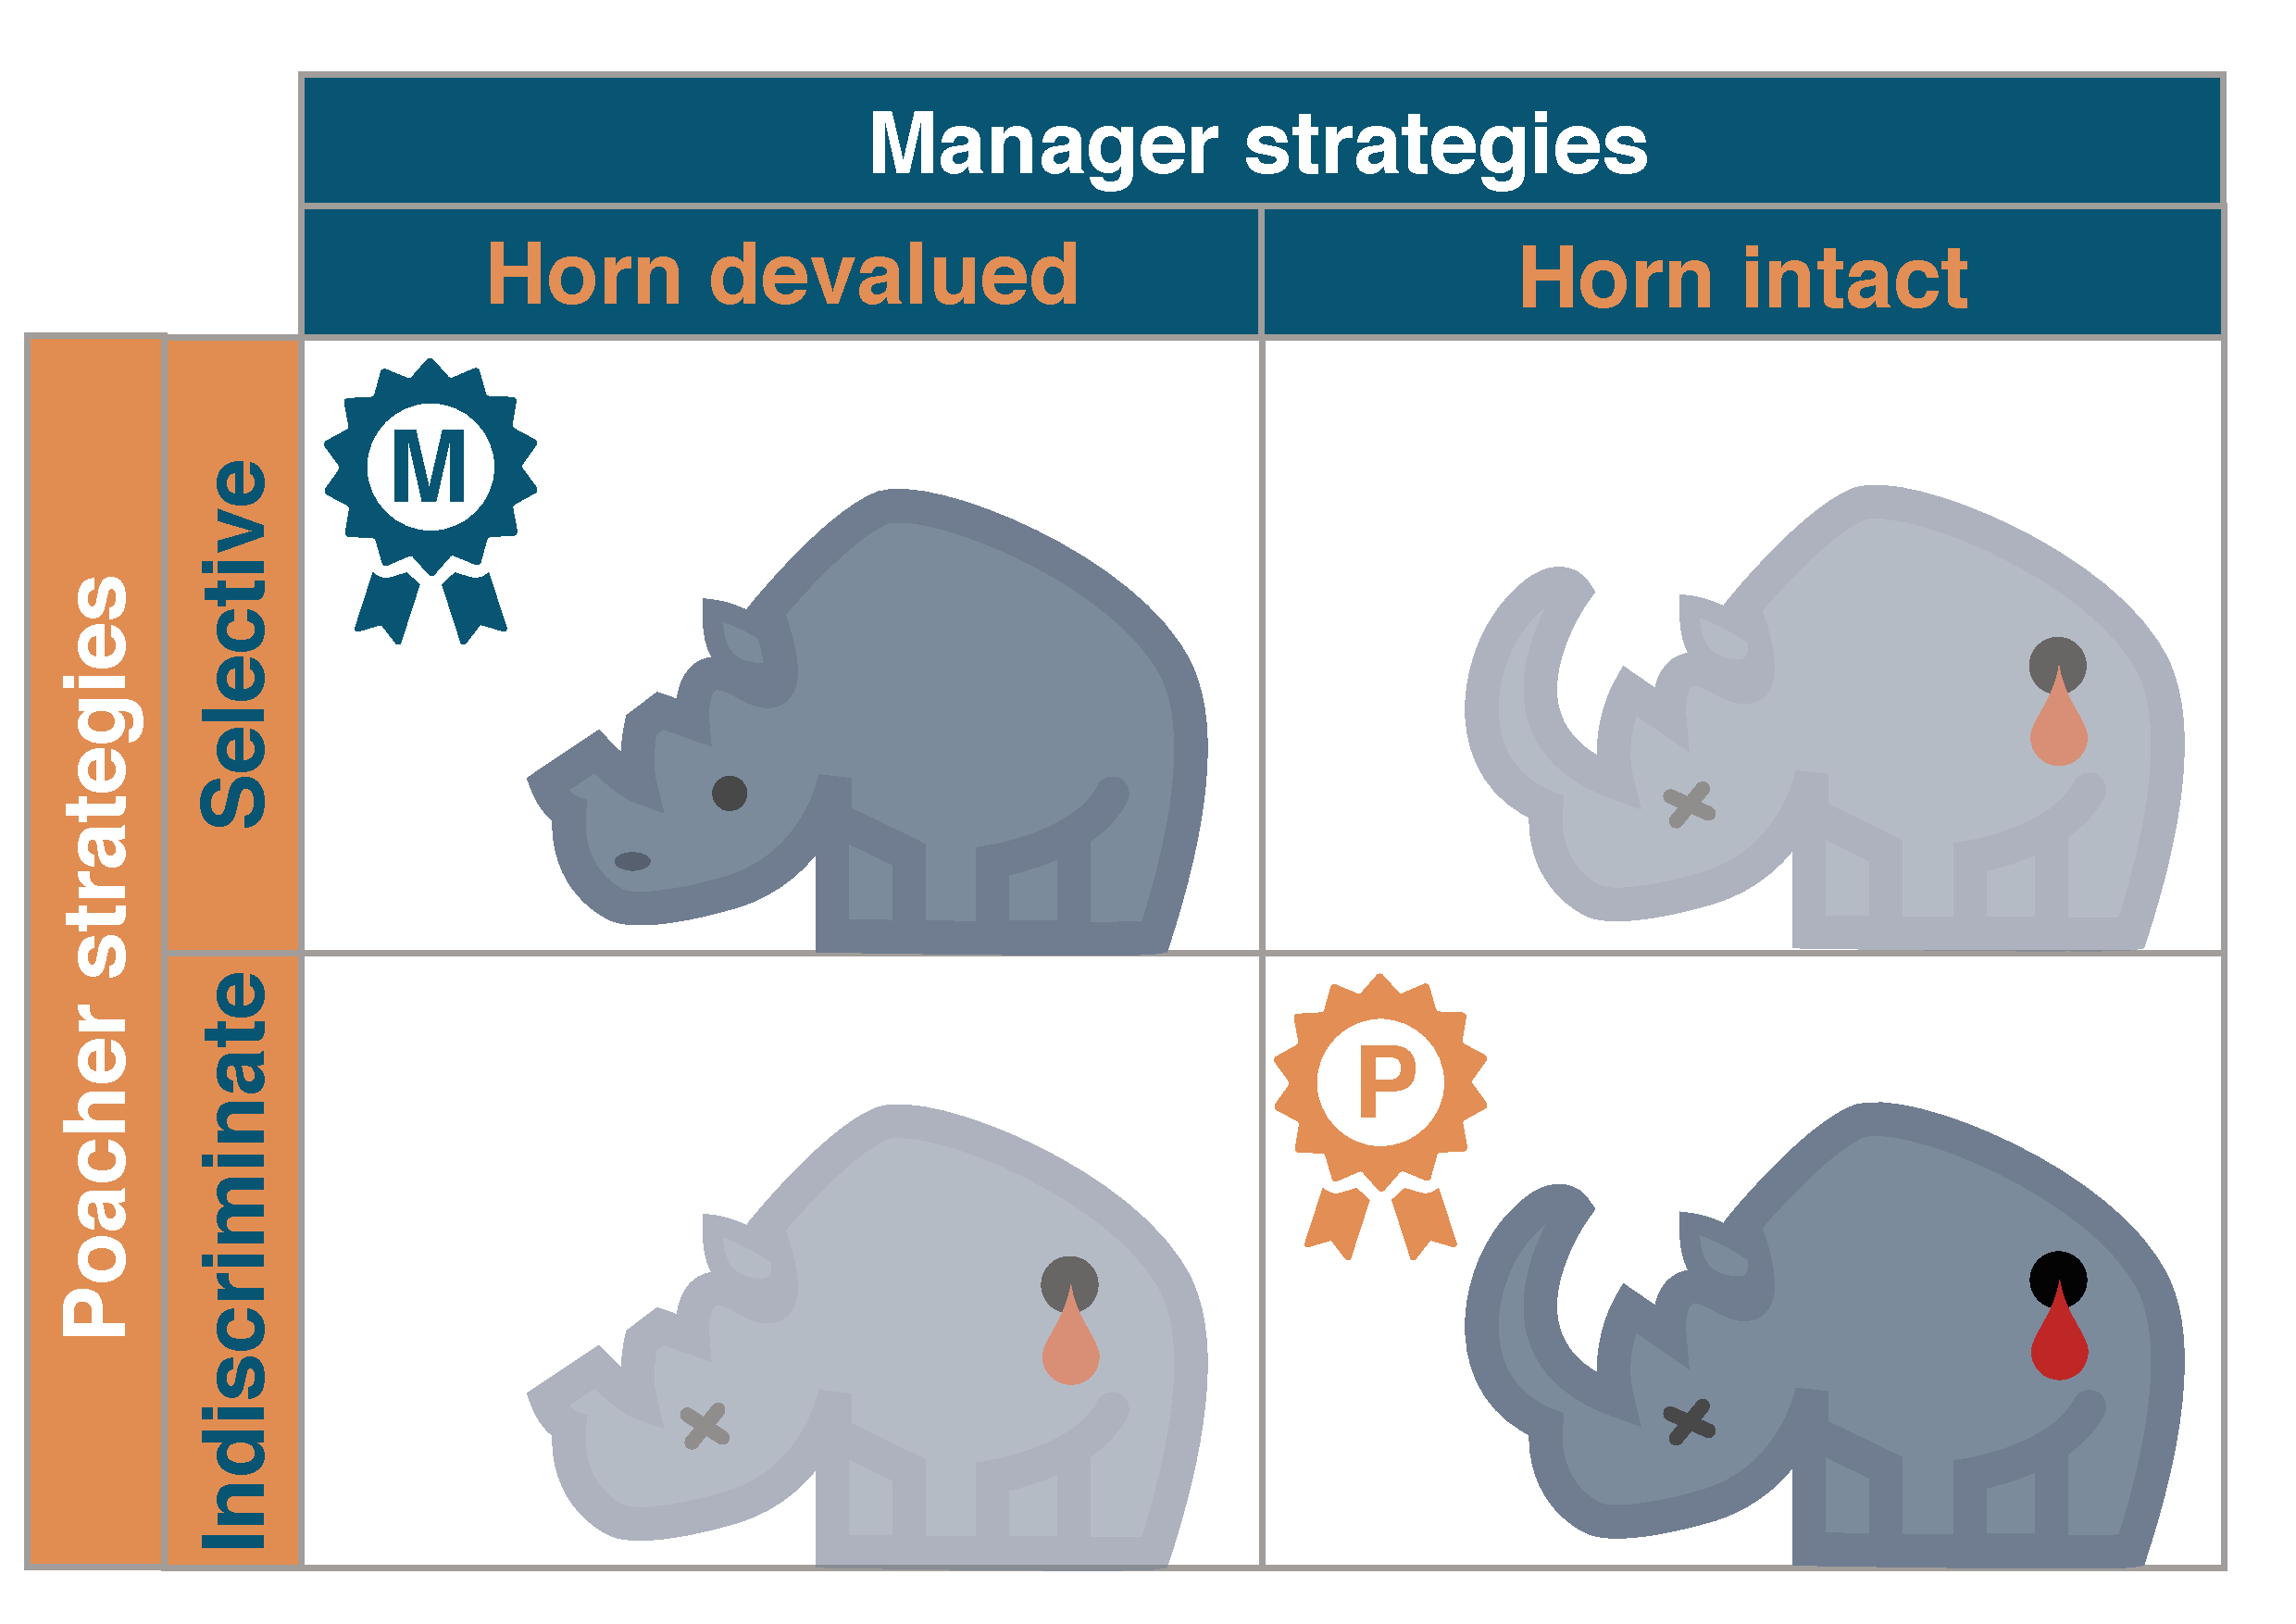
\includegraphics[width=0.5\textwidth]{static/RhinoPic.pdf}\hspace{12pt}
    \includestandalone[width=0.45\textwidth]{static/promotion} \\
    \end{center}
\end{frame}

\begin{frame}
    \begin{center}
    \faTwitter @NikoletaGlyn \\
    
    \vspace{1cm}
    \end{center}

    \footnotesize
    $\bullet$ https://nikoleta-v3.github.io \\
    \faGithub \ \url{github.com/ArcasProject/Arcas} \\
    \faGithub \ \url{github.com/Nikoleta-v3/bibliometric-study-of-the-prisoners-dilemma} \\
    \faGithub \ \url{github.com/Nikoleta-v3/meta-analysis-of-prisoners-dilemma-tournaments} \\
    \faGithub \ \url{github.com/Nikoleta-v3/Memory-size-in-the-prisoners-dilemma} \\
\end{frame}

\end{document}

